% vim: filetype=tex spell

%Helmholtz Cage

\chapter{Helmholtz Cage}

\label{ch:BG}

\Cref{fig:helmholtz} shows a Helmholtz cage that was constructed in 2009 to facilitate testing of systems for the \ac{ARC}. The Helmholtz cage has the ability, under MATLAB control, to generate a magnetic field in any direction.

\begin{figure}[!ht]
    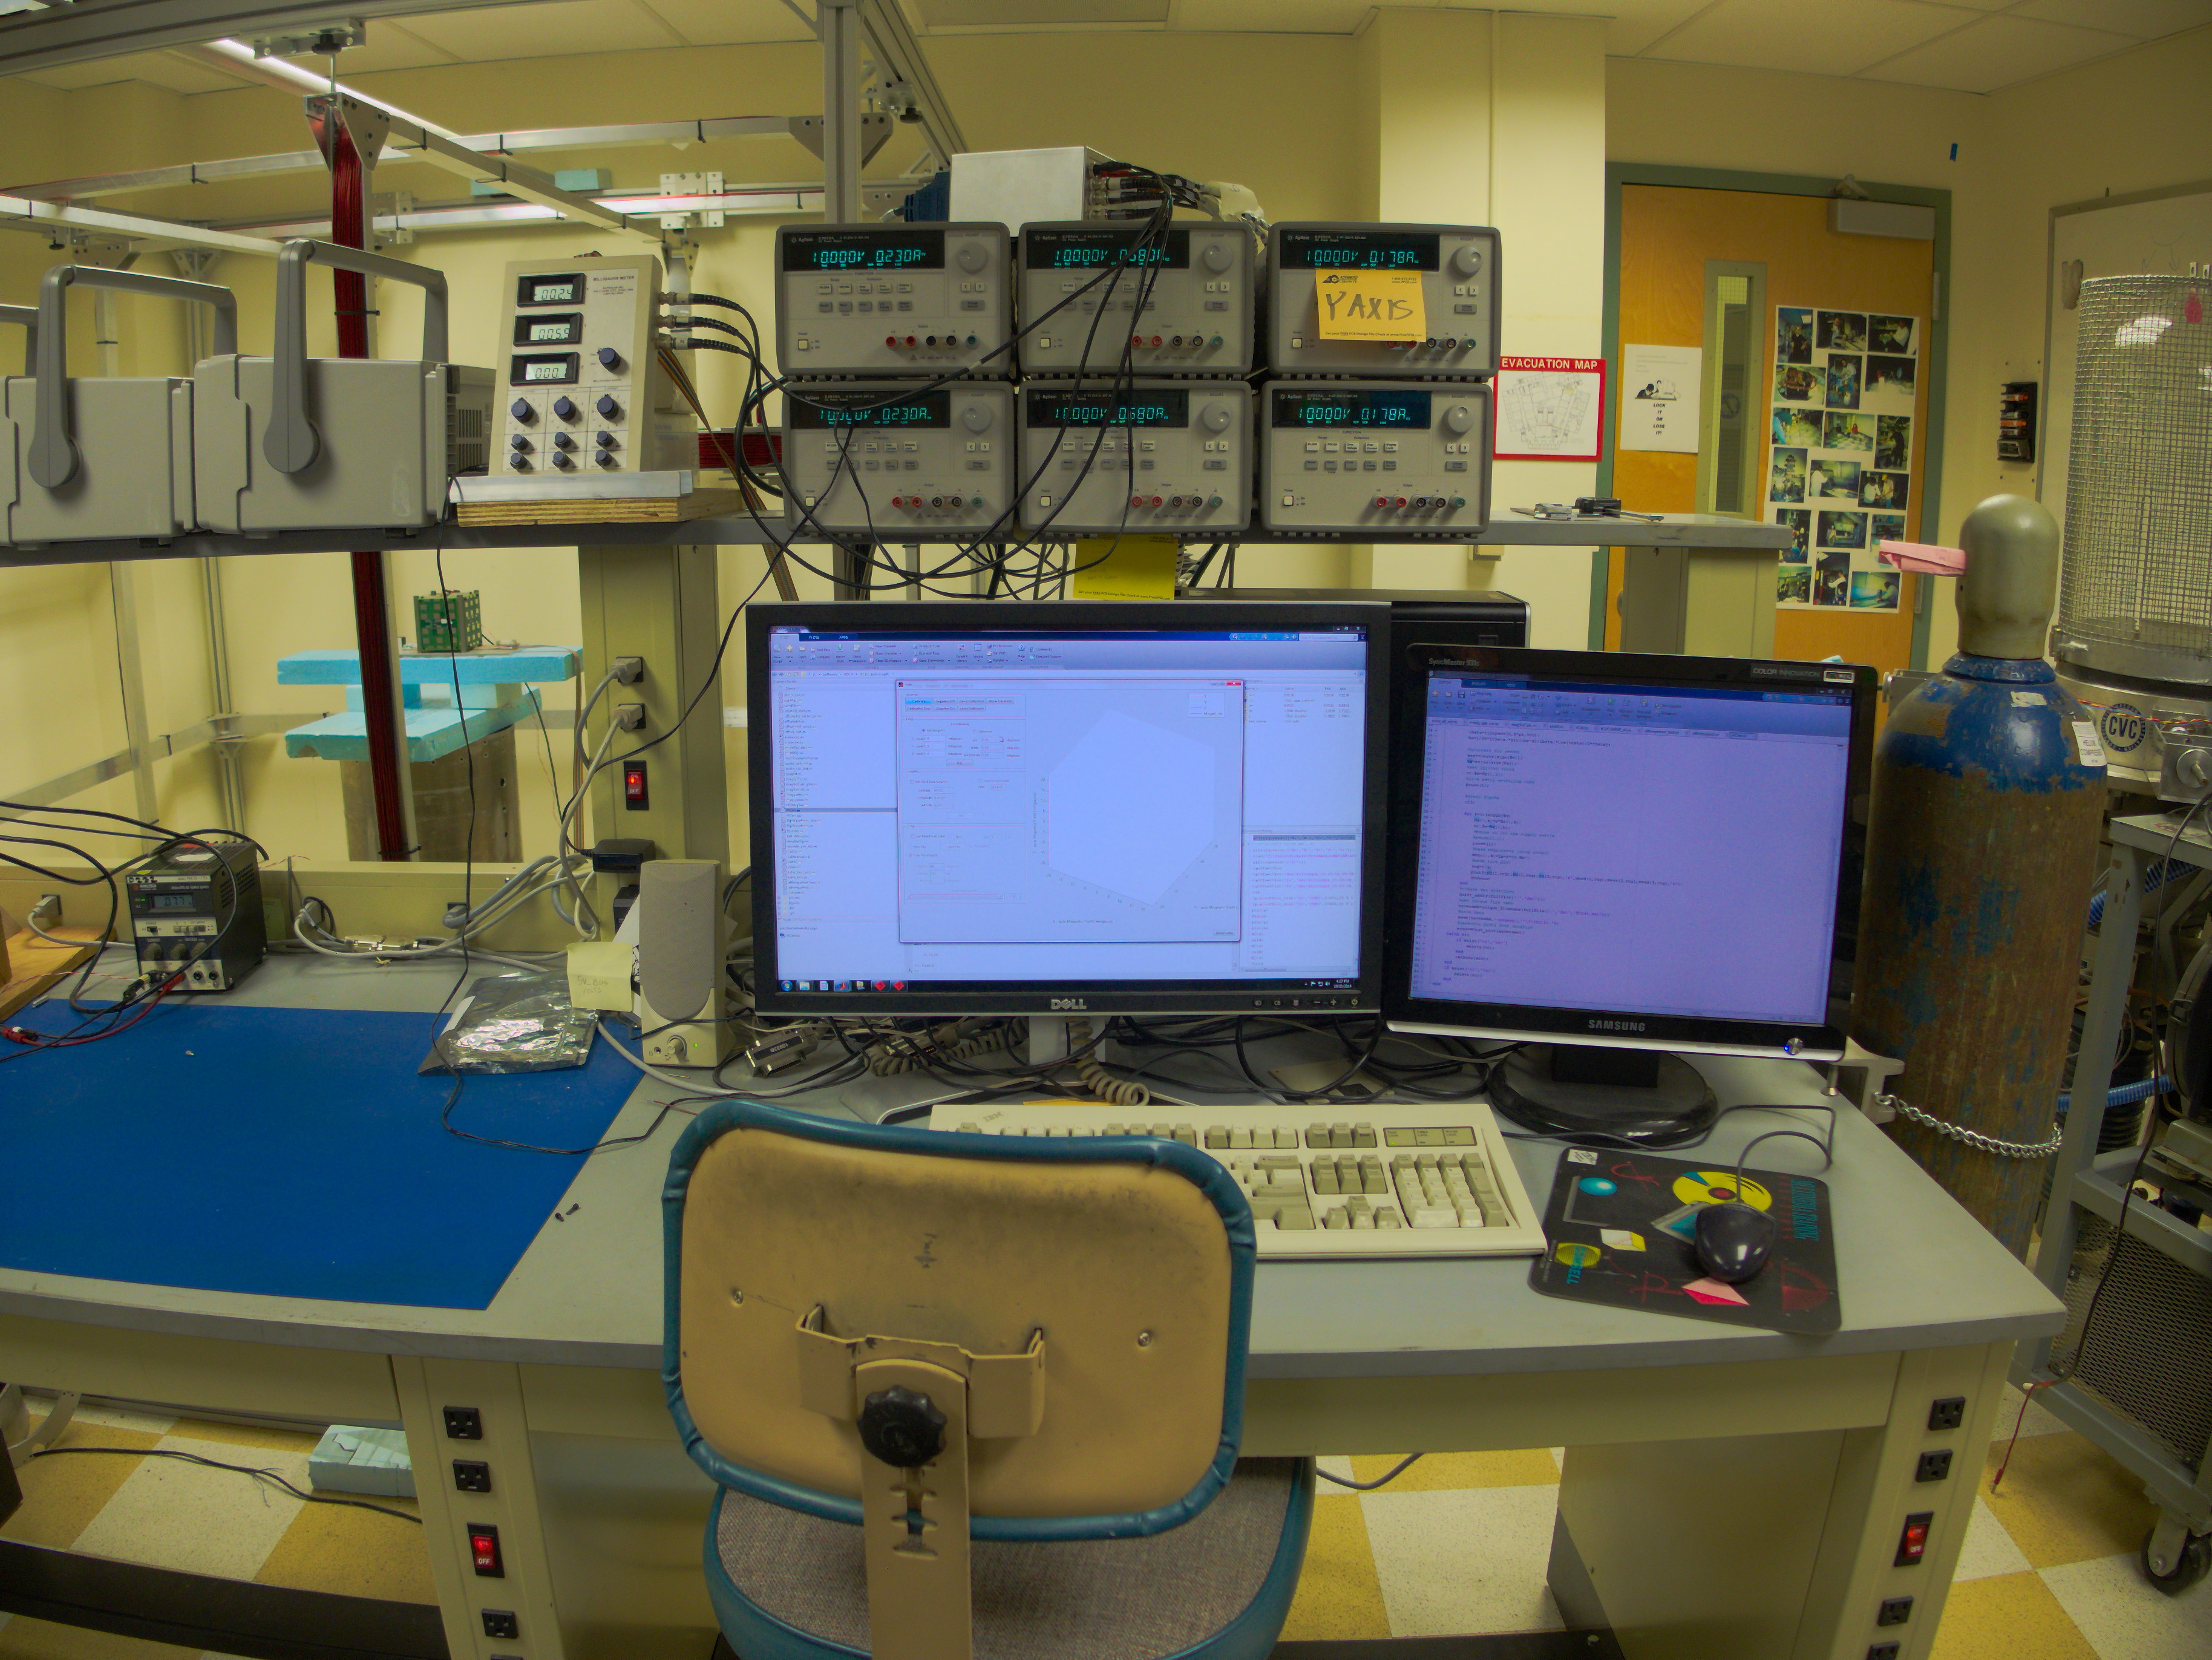
\includegraphics[width=\linewidth]{helmholtz-computer}
    \caption{The Helmholtz cage used for \acs{ACDS} testing}
    \label{fig:helmholtz-comp}
\end{figure}

The computer controlled field allows the calibration and testing process to be automated. The field can be swept through a range of field values and measurements can be taken at each point without human intervention. Once the measurements are complete they can be processed in MATLAB to get immediate results.

\begin{figure}[!ht]
    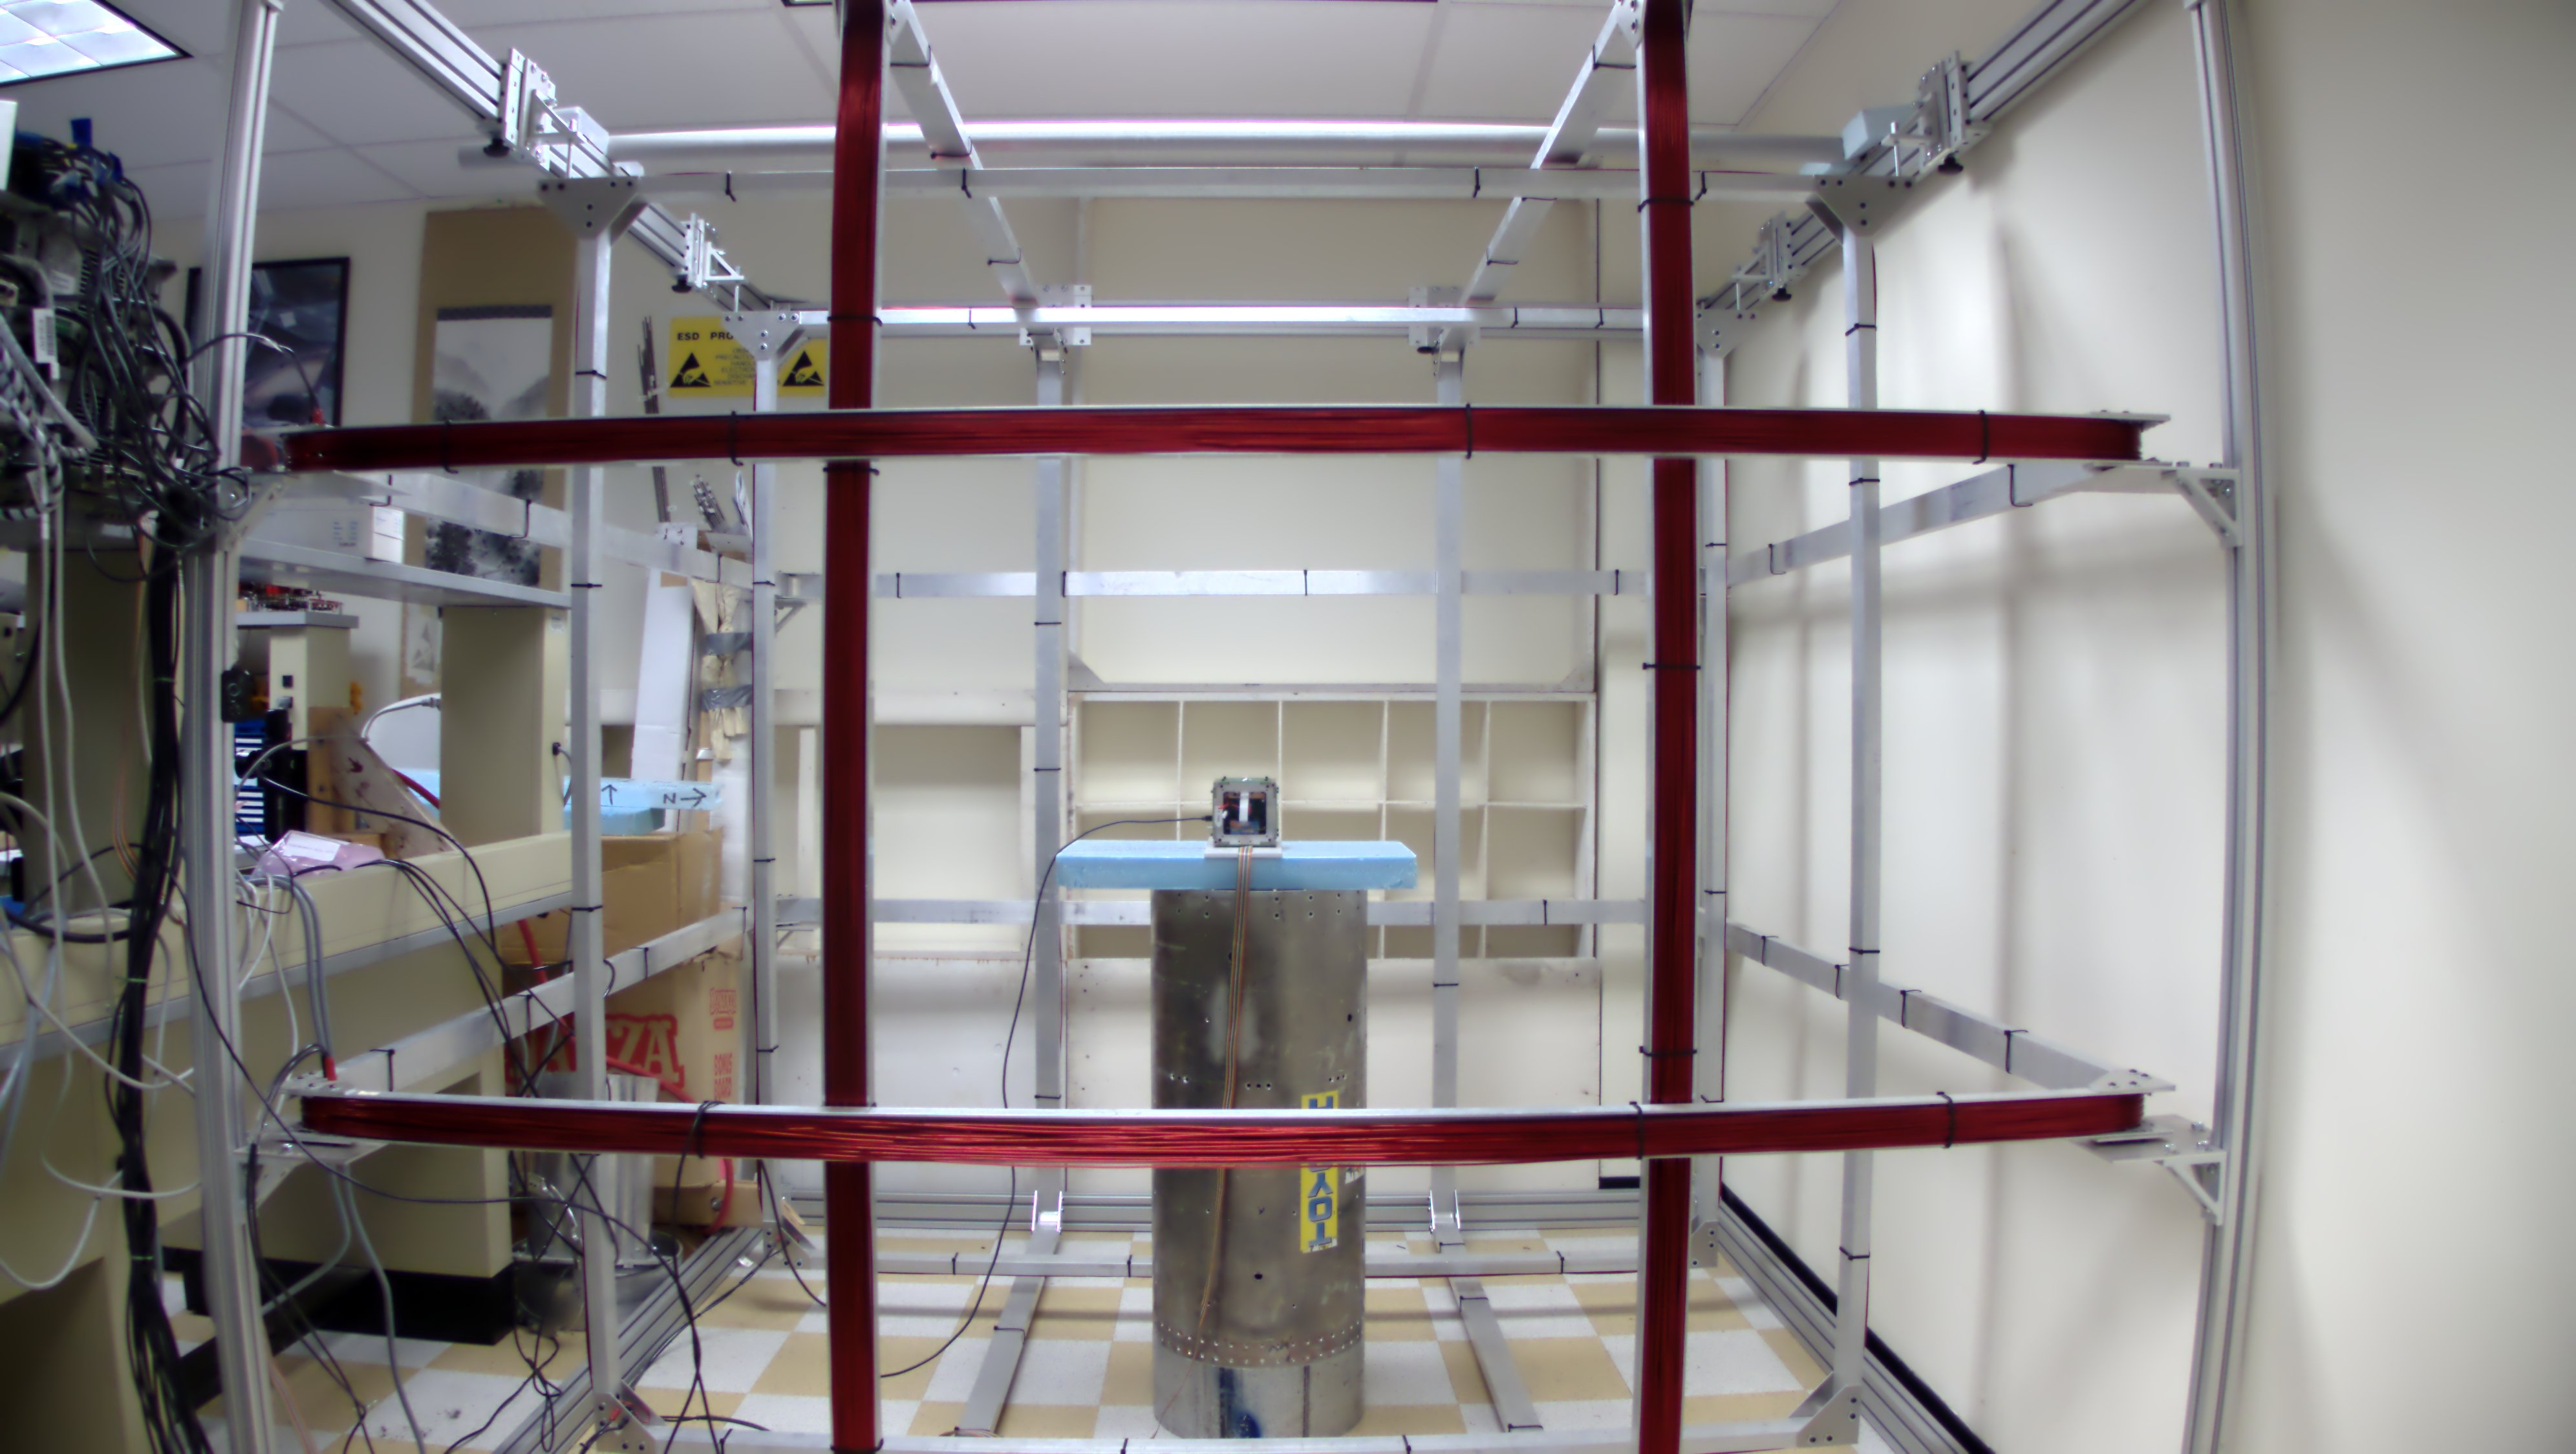
\includegraphics[width=\linewidth]{helmholtz-cage}
    \caption{The Helmholtz cage computer and power supplies}
    \label{fig:helmholtz}
\end{figure}


